\documentclass[11pt,a4j]{jarticle}

\usepackage[dvipdfmx]{graphicx}
\usepackage{amssymb}
\usepackage{amsmath}
\usepackage{ascmac}
\usepackage{setspace}
\usepackage{float}
\usepackage[dvips,usenames,dvipdfmx]{color}
\usepackage{colortbl}
\usepackage{mathtools}
\usepackage{multirow}
\usepackage{algpseudocode}
\usepackage{algorithm}
\usepackage{url}
\usepackage[top=30.5truemm,bottom=30.5truemm,left=22.5truemm,right=22.5truemm]{geometry}
\usepackage{listings}

\renewcommand{\algorithmicrequire}{\textbf{Input:}}
\renewcommand{\algorithmicensure}{\textbf{Output:}}
\algtext*{EndIf}
\algtext*{EndFor}
\algtext*{EndWhile}

\newcommand{\argmin}{\mathop{\rm arg~min}\limits}
\newcommand{\Continue}{\textbf{continue}}
\newcommand{\Break}{\textbf{break}}

\definecolor{bl}{rgb}{0.94,0.97,1}
\definecolor{gr}{rgb}{0.5,0.5,0.5}
\makeatletter
\def\section{\@startsection{section}{1}{\z@}{2.3ex plus -1ex minus -.2ex}{2.3 ex plus .2ex}{\Large\bf}}
\makeatother

\setstretch{1.5}

\usepackage{fancyhdr}
\lhead{\leftmark}
\chead{}
\rhead{\rightmark}
\cfoot{\thepage}

\rfoot{}

\lstset{
  basicstyle={\ttfamily},
  identifierstyle={\small},
  commentstyle={\small\ttfamily \color[rgb]{0,0.5,0}},
  keywordstyle={\small\bfseries \color[rgb]{0,0,0.8}},
  ndkeywordstyle={\small},
  stringstyle={\small\ttfamily \color[rgb]{0,0,1}},
  frame={tb},
  columns=[l]{fullflexible},
  numbers=left,
  xrightmargin=0zw,
  xleftmargin=3zw,
  numberstyle={\scriptsize},
  stepnumber=1,
  numbersep=1zw,
  lineskip=-0.5ex,
  morecomment=[l]{//},
  breaklines=true,
  showstringspaces=\false,
}

\begin{document}
\vspace*{2cm}
\thispagestyle{empty}
% \begin{spacing}{1}
  \begin{center}
    {
      \Large 第4回 AIエッジコンテスト レポート
    } \\[3.5truecm]
    \LARGE
    \Large チーム名 Vertical\_Beach \\
    \Large lp6m, medalotte \\
  \end{center}

  % \clearpage
  % \pagenumbering{roman}
  %               {\fontsize{11pt}{15pt}\selectfont
  %                 \tableofcontents
  %               }
% \end{spacing}

\clearpage
\pagenumbering{arabic}
\pagestyle{fancy}

\section{開発フロー}
DNNのHWアクセラレーションには,Xilinx社から提供されているDPU(Deeplearning Processing Unit)コア\cite{dpuip}および統合開発環境であるVitis-AIを使用した.
Vitis-AIはcaffe,tensorflow等のDNNフレームワークを用いて設計されたDNNモデルを量子化し,DPU向けにデプロイすることができる.\footnote{Vitis-AI v1.3にてpytorchへの一部対応が追加された.}
\section{DNNモデルの学習}
\subsection{DNNモデル}
コンテストの課題であるセマンティックセグメンテーションを行うDNNモデルとして我々はresnet18-FPNを使用した.
モデルはXilinx社から提供されるチュートリアル\cite{tutorial}に含まれるものを流用した.
FPN(Feature Pyramid Network)\cite{fpn}は,低解像だが意味的に強い(semantically strong)特徴と高解像だが意味的に弱い(semantically weak)特徴の両方を使用することで物体検出及び領域分割のタスクにおいて高い精度を挙げられることが知られている.図\ref{figure_fpn}にFPNの概要図を示す.
\begin{figure}[h]
    \begin{center}
        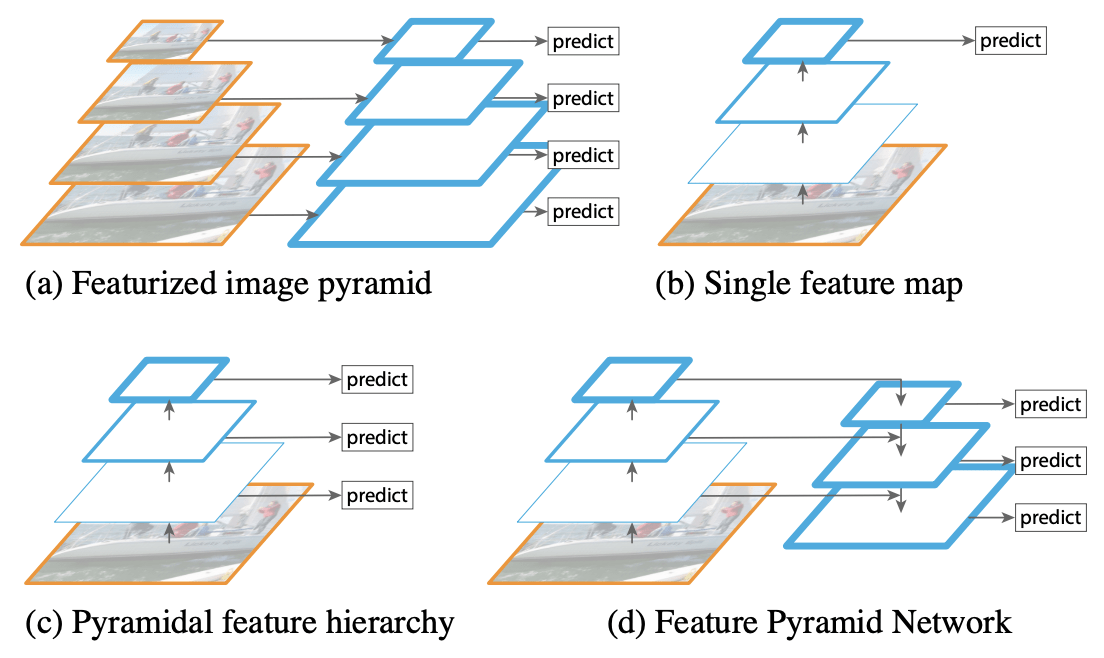
\includegraphics[width=8.0cm]{figures/fpn.png}
        \caption{Feature Pyramid Network\cite{fpn}}
        \label{figure_fpn}
        \end{center}
\end{figure}
\subsection{損失関数}
参考にしたチュートリアルでは損失関数としてSoftmaxWithCrossEntropyが使用されていた.コンテストで提供される学習画像を使用して学習を行ったが,テスト画像に対するmIoUスコアは0.50程度に留まり,処理速度部門における基準値である0.60を上回ることができなかった.
そこで我々は領域分割タスクにおいて精度を向上させる損失関数として提案されているLovasz-Loss関数\cite{lovasz}を採用した.Lovasz-Loss関数は,第1回AIエッジコンテストのセグメンテーション部門において第2位のチームも使用していたことから\cite{ref_signate_report},精度向上に効果的であると考えた.
Lovasz-Lossは予測領域と正解領域のIoUを指標とするJaccard-Lossをさらに拡張したものであり,tensorflowとpytorch向けに公式に実装が公開されている.流用したチュートリアルはCaffeを用いてモデルが定義されており,Caffe上でLovasz-Loss関数を自前で実装するのは困難であった.モデルをpytorchに変換してpytorch上で学習を行い,学習済みの重みをcaffe向けに変換することでこの問題を解消した.
\subsection{学習時の解像度}
推論をFPGAボード上で高速に実行するには,入力画像サイズを小さくしても高い精度が出ることが望ましい.推論時と学習時の解像度が近いほうが精度が向上するのか,あるいは学習時に高解像度の情報を与えるほうが学習精度が向上するのかを検証した.
学習時の入力解像度について以下の2つの方法を比較した.
\begin{itemize}
    \item{512*1024にResize→0.7倍から1.5倍にRandom Scaling→(256*256)にRandom Cropping}
    \item{400*800にResize→0.7倍から1.2倍にRandom Scaling→(256*256)にRandom Cropping}
\end{itemize}
前者では与えられる解像度が(358,716)〜(768,1536)と比較的大きく,後者では(280,560)〜(480,960)と推論時に使用する解像度に近く小さい.比較結果を表\ref{compare_resolution}に示す.今回は後者の方法,すなわち推論時と学習時の解像度が近いほうが精度が僅かに向上する結果となった.
\begin{table}[h]
    \caption{学習時の入力解像度による精度の比較} \vspace{1mm}
    \begin{center}
        \begin{tabular}{lll}
                & Low Resolution & High Resolution \\ \hline
        320*640 & 0.6014         & 0.5829            \\ \hline
        352*704 & 0.6081         & 0.5972               \\ \hline
        384*768 & 0.6121         & 0.6084
        \end{tabular}
    \end{center}
\end{table}
\subsection{学習結果}
\begin{table}[h]
    \caption{損失関数によるmIoUスコア比較} \vspace{1mm}
    \label{compare_resolution}
    \begin{center}
        \begin{tabular}{lc}
            SoftmaxWithCrossEntropy & 0.5093                     \\ \hline
            Lovasz Loss             & 0.6224
        \end{tabular}
    \end{center}
\end{table}
\begin{figure}[h]
    \begin{center}
        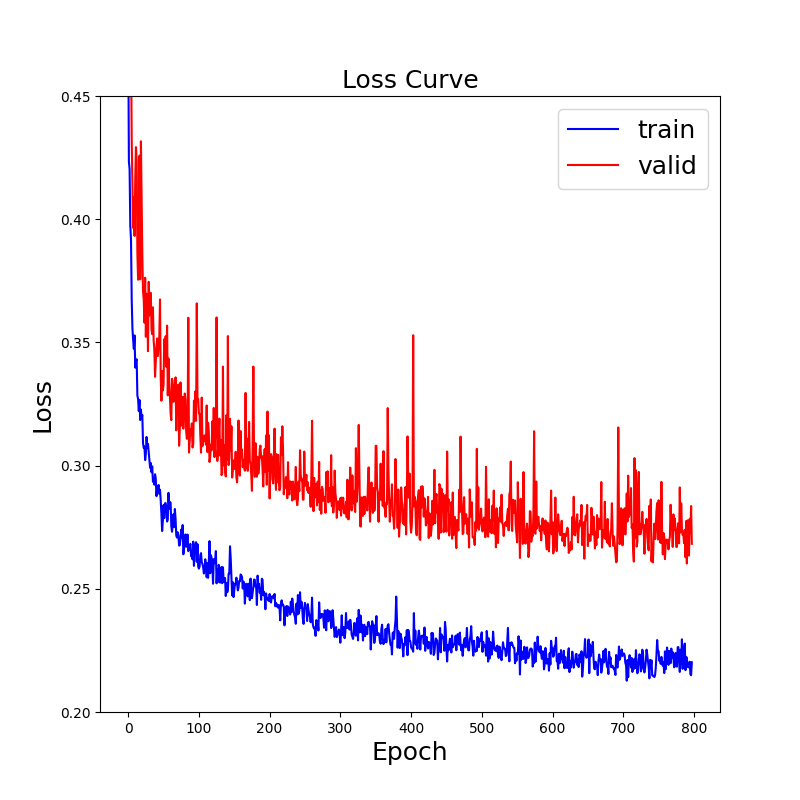
\includegraphics[width=10.0cm]{figures/loss_curve.png}
        \caption{Lovasz-Loss Curve}
        \label{loss_curve}
        \end{center}
\end{figure}
コンテストで提供される学習用画像2243枚の8割を学習用,2割を検証用に分割し学習を行った.
学習した際の学習曲線を図\ref{loss_curve}に示す.
解像度480*960の画像に対してGPU上で推論を行った結果,mIoUスコアは0.62となり,Lovasz-Loss関数を使用したことで精度が大幅に向上した.
\section{ハードウェア最適化}
Xilinx社から提供されるDPU IPコアは,画素や入出力チャネルに対する並列数が異なる複数の種類のIPコアが提供されている.
より並列数の高いIPコアを使用することで処理性能が向上するが,回路規模および消費電力が増加する.
また,DPUコアの一部のレイヤーのサポートを無効にすることでリソース使用率を低減することができる.

コンテストの評価ボードであるUltra96V2に搭載可能なDPUコアとしてB2304を採用した.
デフォルトで有効になっているDepthWiseConvolutionおよびPool Averageのレイヤーは今回設計したモデルでは必要ないため無効にした.

さらに,DPUの動作周波数を高めることにより,DPUにおける推論実行時間を短縮することができる.
論理合成のストラテジをFlow\_AreaOptimized\_high,配置配線のストラテジをperformance\_ExtraTimingOptに変更することで動作周波数を150MHz/300MHzから200MHz/400MHz\footnote{DPUコアはベース周波数に加えてその2倍の周波数のクロックをDSPに接続するため,動作周波数はこのような表記とした.}に高めてもタイミング制約を満たし,FPGAビットストリームの生成を行うことができた.

表\ref{runtimetable}に動作周波数と入力画像サイズごとのDPUにおける推論実行時間・およびスコアを示す.
DPUの推論時間は入力画像サイズに概ね比例し,動作周波数を向上させることによって推論処理が約1.2倍高速化されることがわかる.
\begin{table}[b]
    \label{runtimetable}
    \caption{各入力画像サイズ・動作周波数における推論時間とスコア}
    \begin{center}
        \begin{tabular}{lllll}
            Image Size & \multicolumn{2}{c}{DPUTask {[}ms{]}}                            & \multicolumn{1}{c}{Score} &  \\
                & \multicolumn{1}{r}{150/300MHz} & \multicolumn{1}{r}{200/400MHz} &                           &  \\ \hline
        256*512 & 35                             & 30                             & 0.539                     &  \\ \hline
        320*640 & 60                             & 55                             & 0.579                     &  \\ \hline
        352*704 & 72                             & 65                             & 0.593                     &  \\ \hline
        384*768 & 81                             & 70                             & 0.608                     &  \\ \hline
        480*960 & 128                            & 110                            & 0.616                     & 
        \end{tabular}
    \end{center}
\end{table}

\section{ソフトウェア最適化}
本コンテストでは 1216x1936 の車載カメラ画像の Semantic Segmentation を行うことが課題として設定されている.
具体的には,入力画像の各ピクセルに対して4カテゴリ (乗用車,歩行者,信号,車道・駐車場)
の分類を行った結果を出力する推論アプリケーションの実装が求められる.

我々の実装では,
入力画像の縮小 (1216x1936 $\rightarrow$ 320x640) ,および,正規化を行った後にDPUによる推論を行う.
また,DPUによる推論の結果は,ラベル付け,および,入力画像と同サイズへの拡大 (320x640 $\rightarrow$ 1216x1936) を行うことで出力画像となる.
ところで,本コンテストのルールでは,入力画像のメモリ上へのロード,および,出力画像のファイル出力は推論処理時間に含めない.
よって,上記の前処理(縮小・正規化),推論(DPU実行),後処理(ラベル付け・拡大)の3つの処理が推論処理時間計測の対象となる.

我々はこれらの処理のマルチスレッド実装を行った.
DPUによる推論の実行中に,次の画像の前処理,および,前の画像の後処理を行うことで,
シーケンシャルに処理する場合に比べて大幅な高速化が見込まれる.

本章では,はじめに上記の処理をシングルスレッド実装する場合についての説明を行う.
その後,マルチスレッド実装についての説明を行う.

\subsection{シングルスレッド実装}
図 \ref{fig:singlethread} に我々の推論処理をシングルスレッドで実装する場合のフローチャートを示す.

\begin{figure}[h]
  \begin{center}
    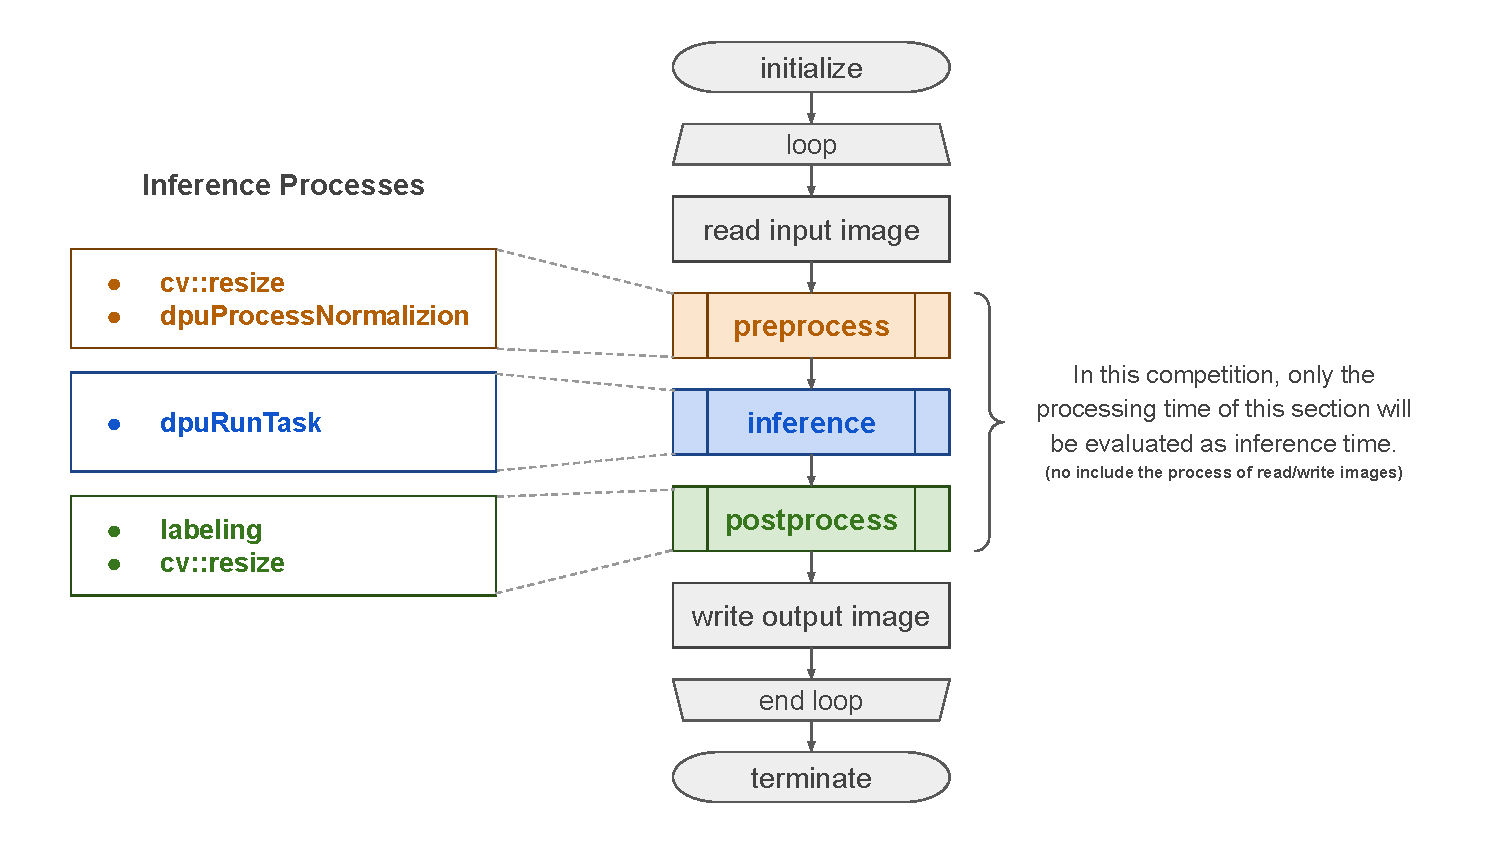
\includegraphics[width=\linewidth]{figures/sw_opt_flowchart_singlethread.pdf}
    \caption{シングルスレッド実行時}
    \label{fig:singlethread}
  \end{center}
\end{figure}

シングルスレッド実装を行う場合,
画像を1枚読み込み,推論を行い,推論結果を書き込む処理をテスト画像全てに対して繰り返す実装が考えられる.
前処理(preprocess),推論処理(inference),後処理(postprocess)の実行区間が推論処理時間計測の対象である.
前処理では,OpenCVの関数cv::resizeを用いて入力画像の縮小を行い,
Vitis-AIのDPUライブラリの関数dpuProcessNormalizionによって各画素値の正規化を行う.
推論処理では,DPUによる推論を行う関数dpuRunTaskを実行する.
後処理では,推論結果を参照してラベル画像を生成し,
その後,関数cv::resizeを用いてラベル画像の拡大を行う.

\subsection{マルチスレッド実装}
今回我々が実装したマルチスレッド実装の概要を図 \ref{fig:multithread} に示す.

\begin{figure}[h]
  \begin{center}
    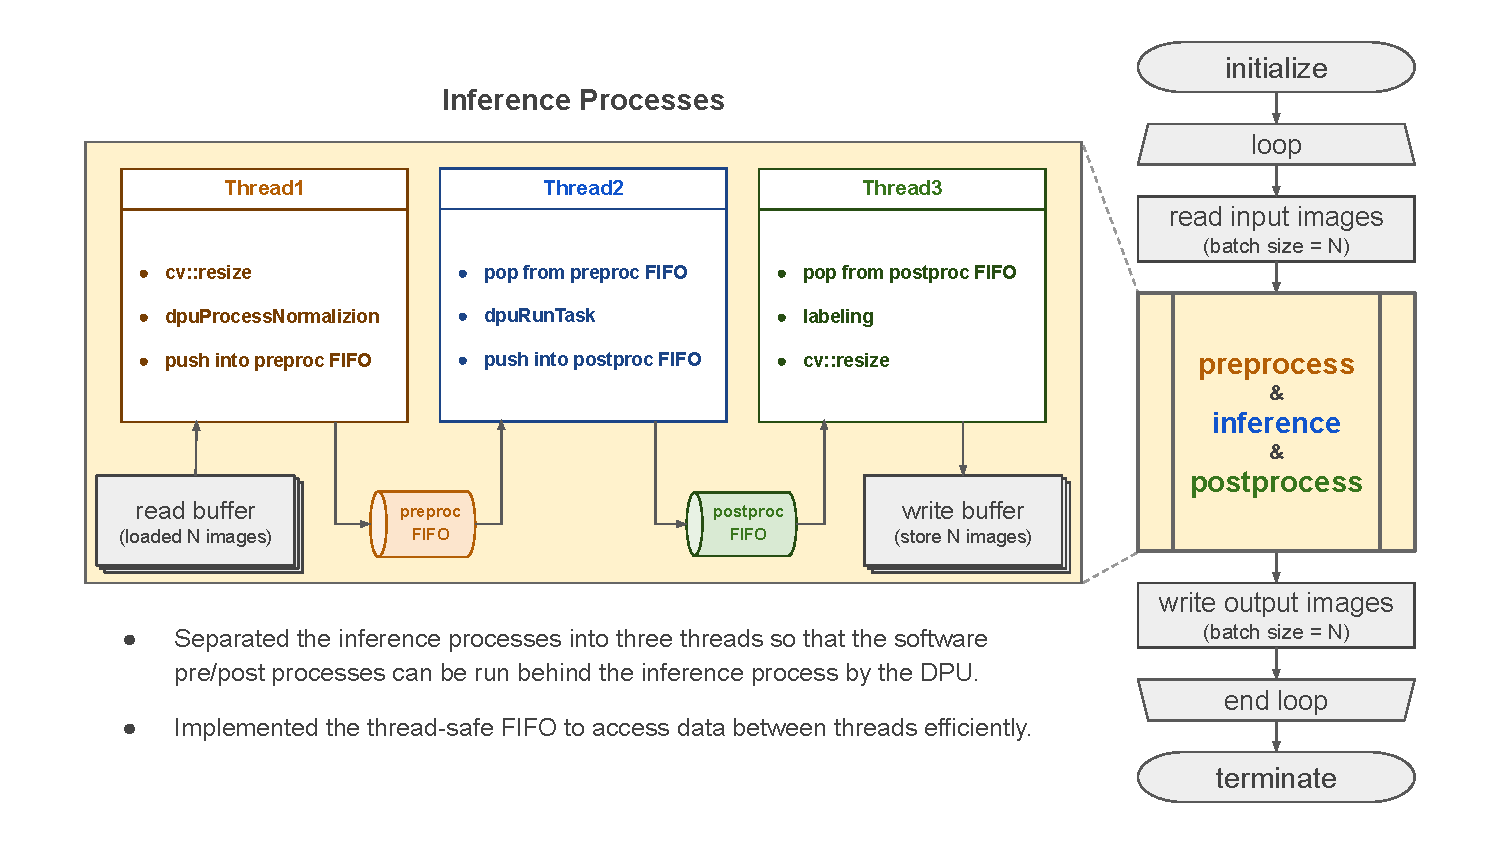
\includegraphics[width=\linewidth]{figures/sw_opt_flowchart_multithread.pdf}
    \caption{マルチスレッド実行時}
    \label{fig:multithread}
  \end{center}
\end{figure}

我々のマルチスレッド実装では,前処理,推論処理,後処理をそれぞれ別スレッド(Thread1, Thread2, Thread3)で実行する.
スレッドセーフなFIFOクラスを実装し,
これを用いてスレッド間でデータを受け渡す実装を行った.
前処理を行うスレッドで処理したデータを推論処理を行うスレッドに渡すpreproc FIFOと,
推論処理を行うスレッドで得られた結果を後処理を行うスレッドに渡すpostproc FIFOの2つを用いる.
また,マルチスレッド実装では1枚ずつ推論を行うのではなく,複数枚の画像のバッチ処理を行う.
ここでは一度のバッチ処理に使用する入力画像の枚数を $N$ とする.
このような実装により,前処理,推論処理,後処理がソフトウェア的にパイプライン処理され,
実行速度の向上が期待される.

図 \ref{fig:sequence} にマルチスレッド実装における処理のシーケンス図を示す.

\begin{figure}[h]
  \begin{center}
    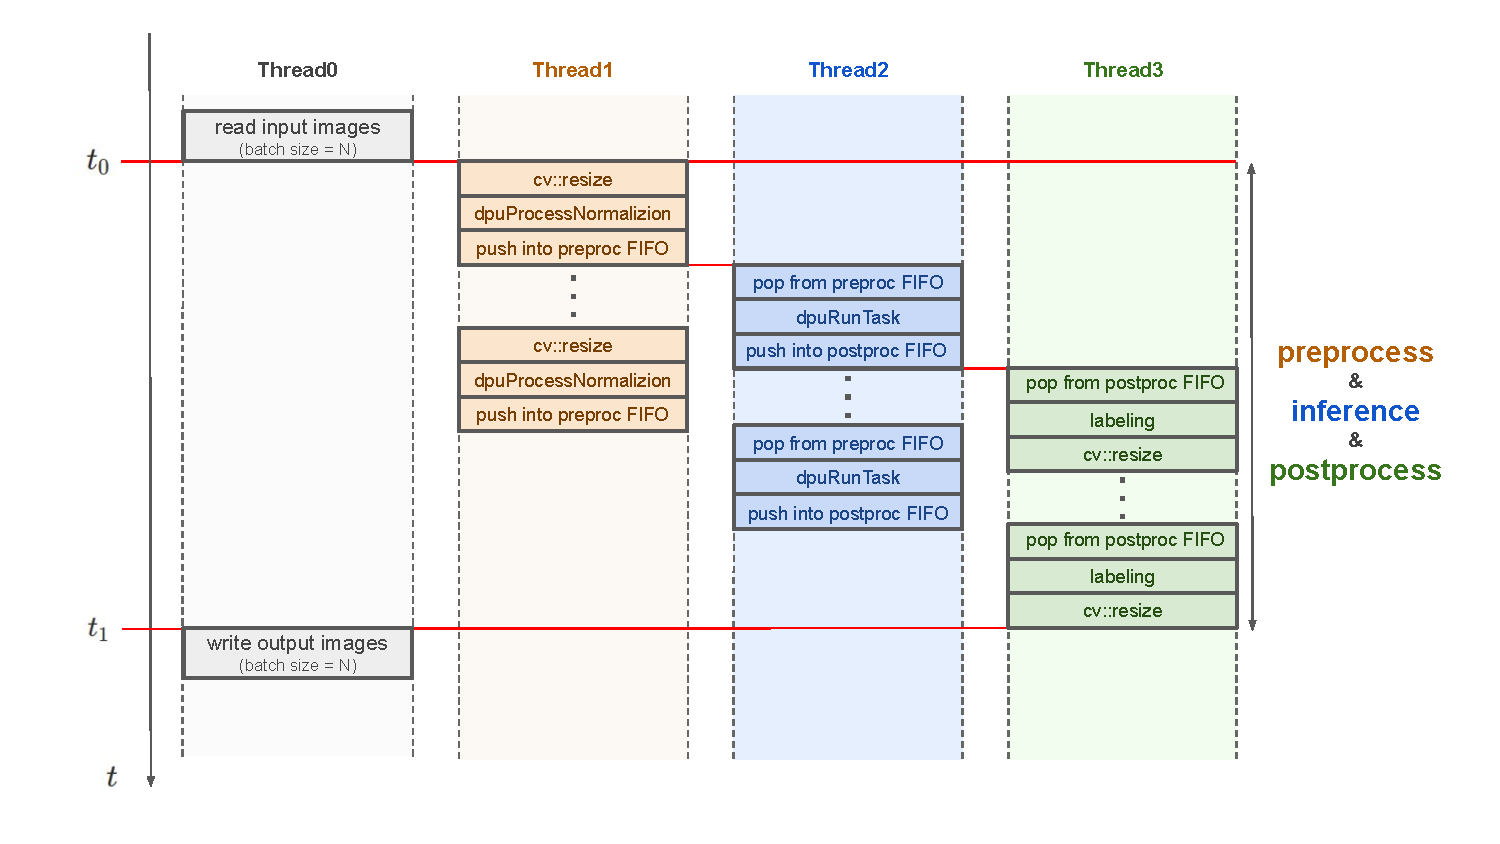
\includegraphics[width=\linewidth]{figures/sw_opt_sequence.pdf}
    \caption{シーケンス図}
    \label{fig:sequence}
  \end{center}
\end{figure}

この図では, $N$ 枚の画像をメモリ上に読み込み,推論を行った後に結果をファイル出力するまでの期間を示している.

\subsubsection{前処理}

\setcounter{lstnumber}{1}
\begin{lstlisting}[language=c++,firstnumber=last,caption=do\_preprocess(),label=code:preproc,float,floatplacement=H]
void do_preprocess() {
  cv::Mat in(in_size, CV_8UC3);
  auto r_buf = read_buffer.begin();
  auto end = false;
  while (!end) {
    cv::resize(*r_buf, in, in.size(), 0, 0, cv::INTER_LINEAR);
    end = (bool)(r_buf == read_buffer.end())
    preproc_fifo.write(ok, end, [&](PreprocFIFOElementType& dst) -> void {
      dpuProcessNormalizion(dst.data(), in.data, in.rows, in.cols, in_mean, in_scale_fix, in.step1());
    });
    r_buf++;
  }
}
\end{lstlisting}

\subsubsection{推論処理}

\setcounter{lstnumber}{1}
\begin{lstlisting}[language=c++,firstnumber=last,caption=do\_inference(),label=code:inference,float,floatplacement=H]
void do_inference() {
  constexpr auto in_size  = sizeof(int8_t) * IN_IMG_W * IN_IMG_H * IN_IMG_C;
  constexpr auto out_size = sizeof(int8_t) * OUT_IMG_W * OUT_IMG_H * NOF_CLASS;
  auto end = false;
  while (!end) {
    preproc_fifo.read(ok, [&](const PreprocFIFOElementType& src) -> void {
      std::memcpy(in_addr, src.data(), in_size);
    });
    dpuRunTask(task_conv_1);
    end = preproc_fifo.neverReadNextElement();
    postproc_fifo.write(ok, end, [&](PostprocFIFOElementType& dst) -> void {
      std::memcpy(dst.data(), out_addr, out_size);
    });
  }
}
\end{lstlisting}

\subsubsection{後処理}

\setcounter{lstnumber}{1}
\begin{lstlisting}[language=c++,firstnumber=last,caption=do\_postprocess(),label=code:postproc,float,floatplacement=H]
void do_postprocess() {
  cv::Mat out(out_size, CV_8UC1);
  auto w_buf = write_buffer.begin();
  while (postproc_fifo.neverReadNextElement()) {
    postproc_fifo.read(ok, [&](const PostprocFIFOElementType& dst) -> void {
      auto offset = dst.data();
      for (int ri = 0; ri < out.rows; ri++) {
        for (int ci = 0; ci < out.cols; ci++) {
          const auto max_itr = std::max_element(offset, offset + NOF_CLASS);
          out.at<uint8_t>(ri, ci) = (uint8_t)(std::distance(offset, max_itr));
          offset += NOF_CLASS;
        }
      }
    });
    cv::resize(out, *w_buf, (*w_buf).size(), 0, 0, cv::INTER_NEAREST);
    w_buf++;
  }
}
\end{lstlisting}

\section{性能評価}
コンテストから提供されるテスト画像649枚に対してUltra96-V2ボード上で推論を実行した.
実行時間の評価における設定項目は以下の通りである.
\begin{description}
  \item[DPU:] B2304@200/400MHz
  \item[推論画像サイズ:] 320*640
  \item[$N$ (一度に処理する画像の数):] 130
\end{description}
\subsection{実行時間}
テスト用画像 649 枚に対する推論処理時間の平均を計測した.
はじめにシングルスレッド実装における詳細な処理時間を表 \ref{tbl:time-singlethread} に示す.

\begin{table}[h]
  \caption{シングルスレッド実装における平均処理時間} \vspace{1mm}
  \label{tbl:time-singlethread}
  \begin{center}
    \begin{tabular}{cc}
      name & elapsed time (ms) \\ \hline
      $t_{\mathrm{pre\_resize}}$    & 9.36 \\ \hline
      $t_{\mathrm{pre\_normalize}}$ & 1.98 \\ \hline
      $t_{\mathrm{pop}}$            & 0.63 \\ \hline
      $t_{\mathrm{dpu}}$            & 54.1 \\ \hline
      $t_{\mathrm{push}}$           & 1.09 \\ \hline
      $t_{\mathrm{post\_labeling}}$ & 6.93 \\ \hline
      $t_{\mathrm{post\_resize}}$   & 5.25 \\ \hline
    \end{tabular}
  \end{center}
\end{table}

シングルスレッド実装では,
前処理の平均処理時間($t_{\mathrm{pre\_resize}} + t_{\mathrm{pre\_normalize}}$)は11.3ms,
DPUによるによる推論の平均処理時間($t_{\mathrm{dpu}}$)は54.1ms,
後処理の平均処理時間($t_{\mathrm{post\_labeling}} + t_{\mathrm{post\_resize}}$)は12.2msであった.
シングルスレッド実装の推論平均処理時間はこれらの合計値,すなわち,77.7msであることが分かる.

マルチスレッド実装では,
推論平均処理時間($t_{\mathrm{inference}}$)が57.9msとなった.
処理のマルチスレッド化により約25\%の高速化を達成したことが分かる.
ここで,マルチスレッド化によるオーバーヘッド $t_\alpha$ は1.93msであった.

\subsection{実行結果}

図 \ref{estimate_result} に入力画像と推論結果,および推論結果を入力画像に合成したものの1例を示す.

\begin{figure}[h]
  \begin{center}
    \caption{推論結果}
    \begin{minipage}{0.32\hsize}
      \begin{center}
        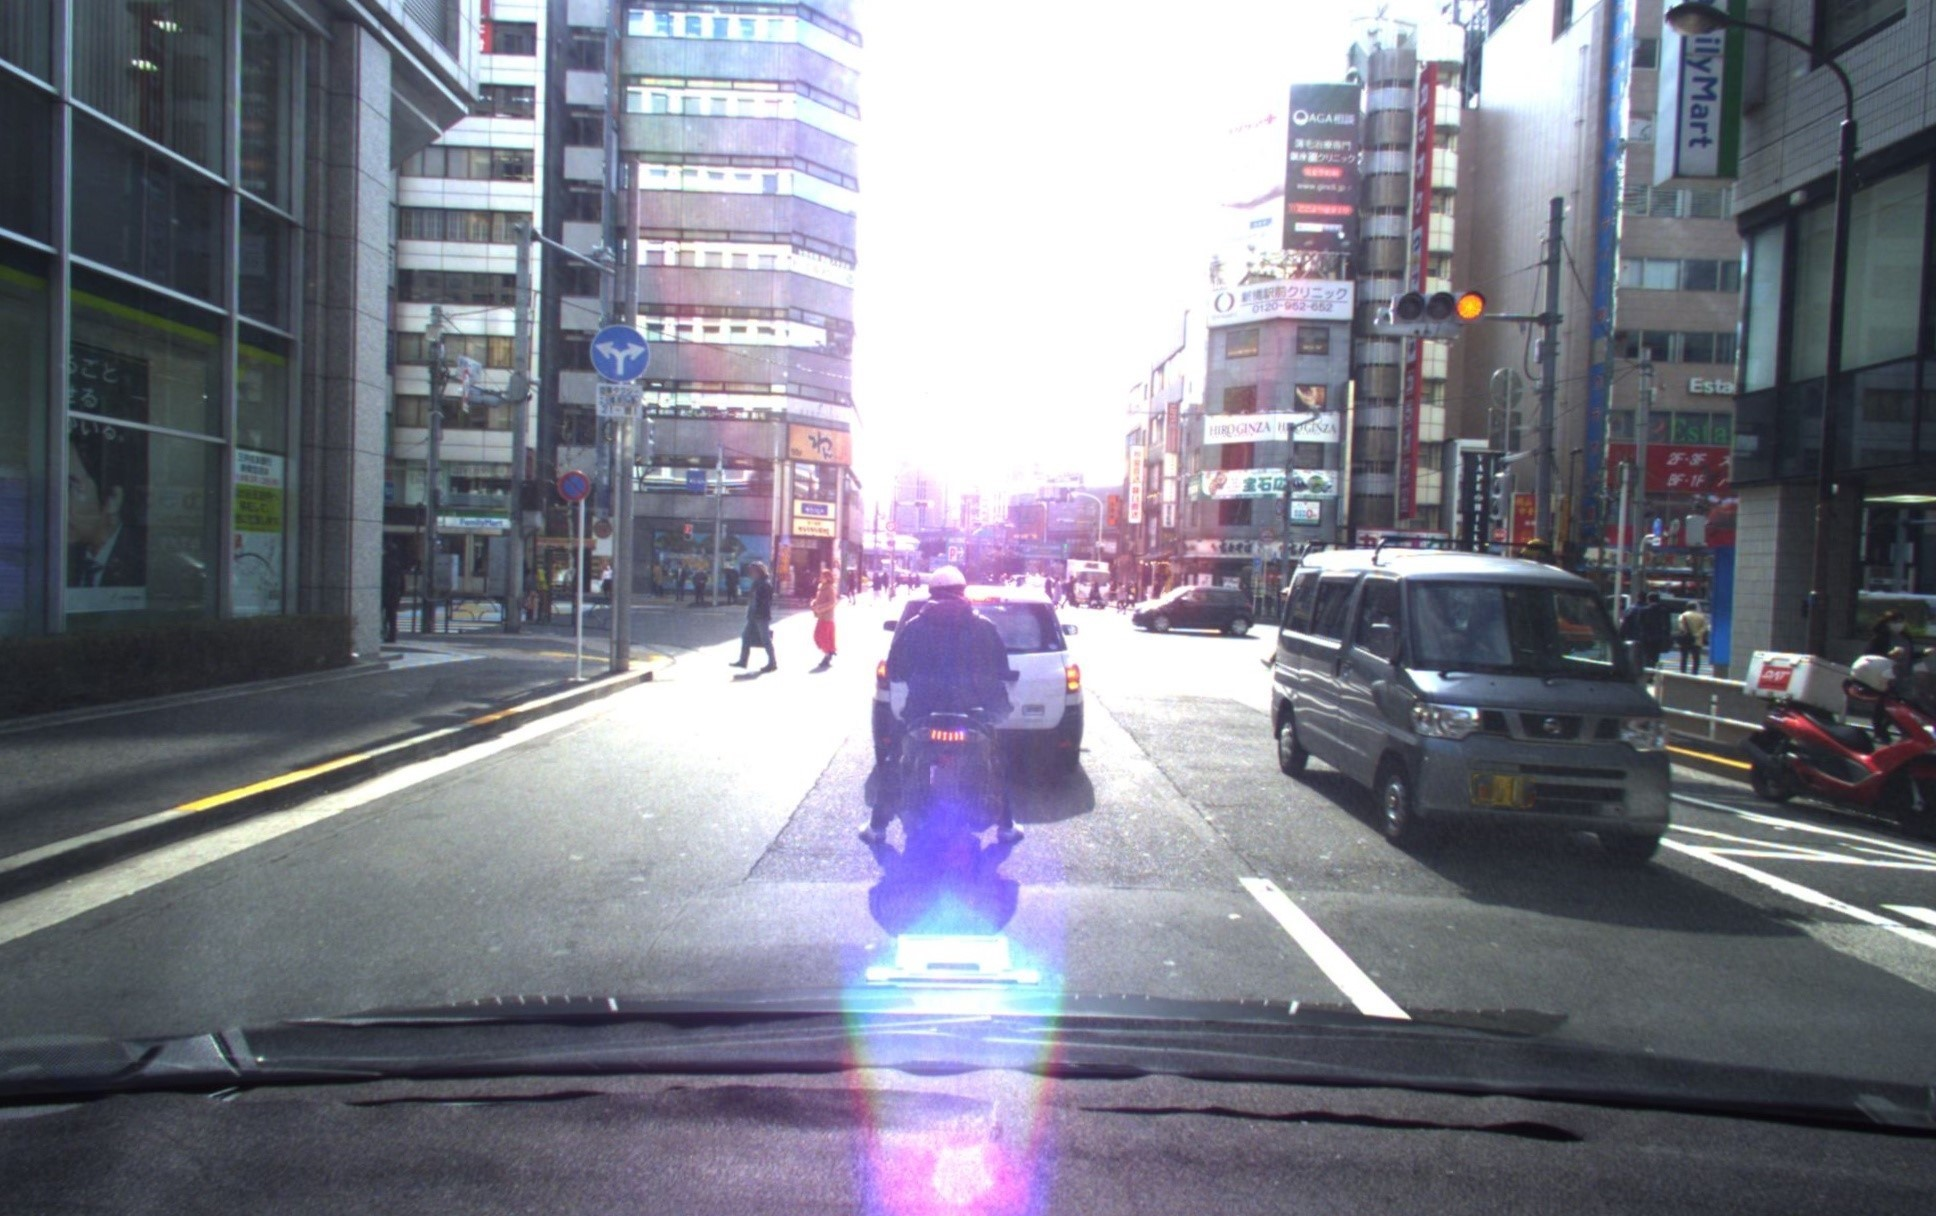
\includegraphics[width=\linewidth]{./figures/orig.jpg}
      \end{center}
    \end{minipage}
    \begin{minipage}{0.32\hsize}
      \begin{center}
        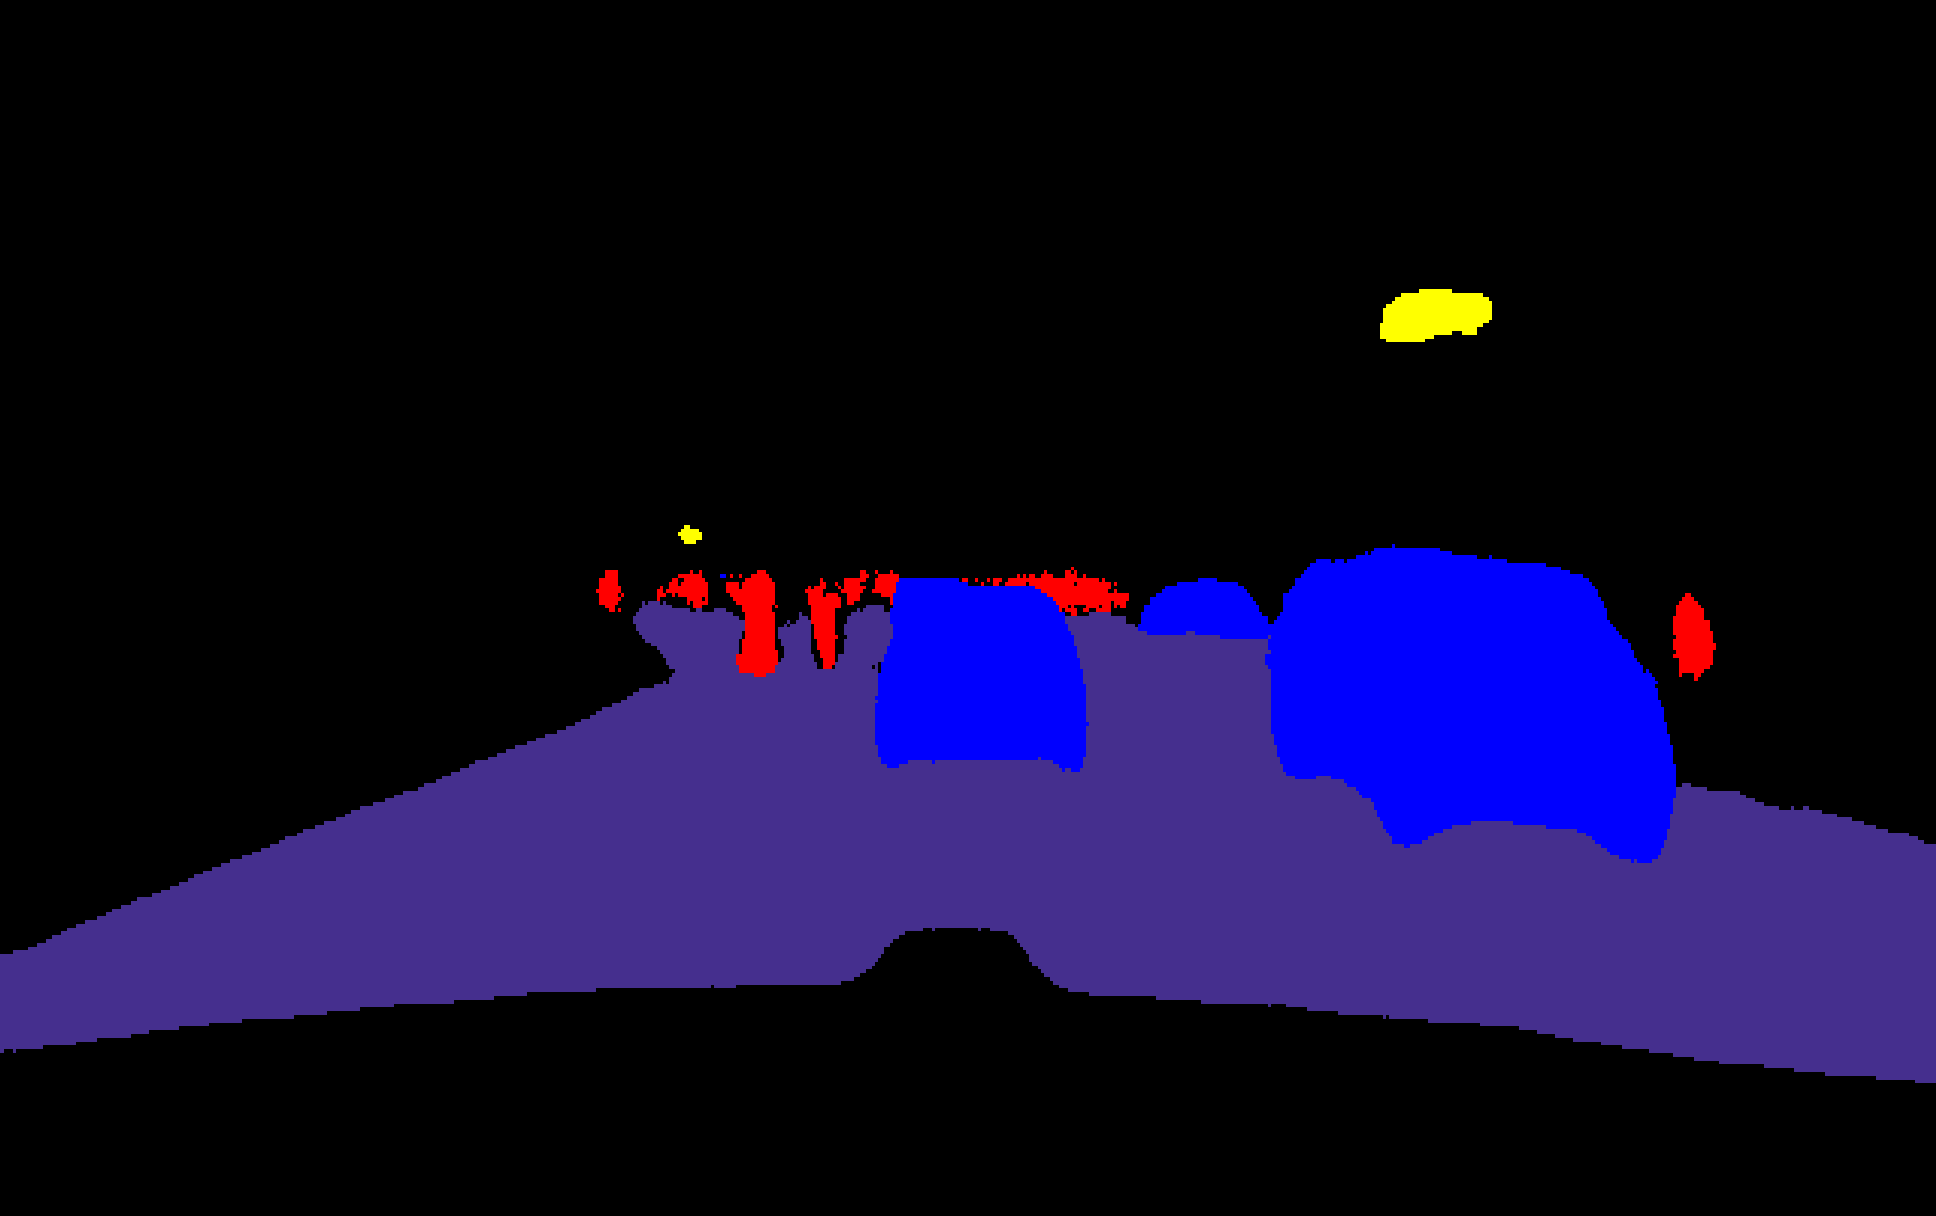
\includegraphics[width=\linewidth]{./figures/label.png}
      \end{center}
    \end{minipage}
    \begin{minipage}{0.32\hsize}
      \begin{center}
        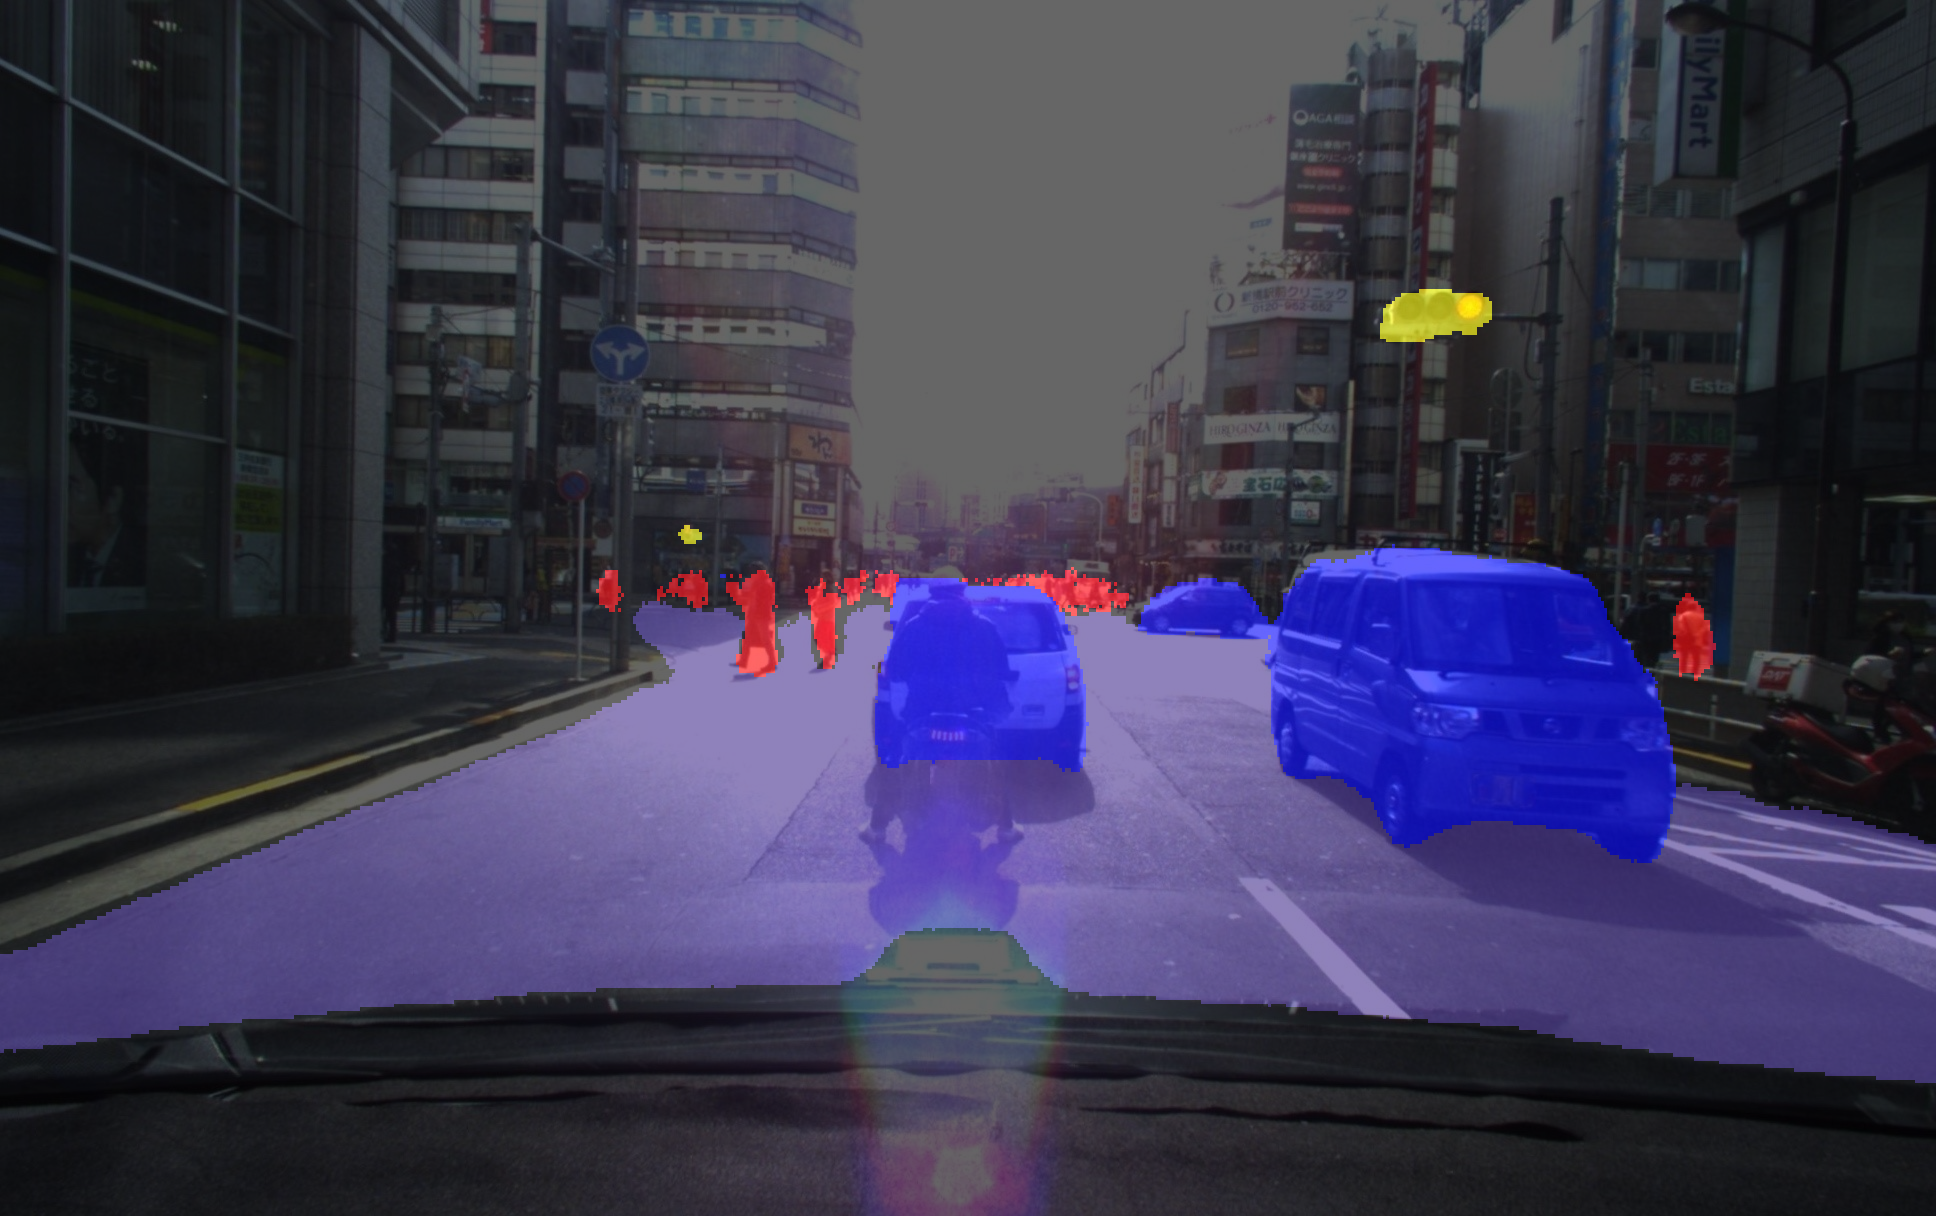
\includegraphics[width=\linewidth]{./figures/mixed.png}
      \end{center}
    \end{minipage}
    \label{estimate_result}
  \end{center}
\end{figure}
推論結果をSIGNATEに投稿した結果,mIoUスコアは0.6014857となった.

\subsection{リソース使用率}
B2304 DPUを第3章で説明したとおりのコンフィグレーションで実装した場合のDPUおよび回路全体のリソース使用率を表\ref{resource_util}に示す.
DPU IPを含んだVivadoプロジェクトをVitisが自動生成する際にベースとするプラットフォームプロジェクトにAXI GPIOやUARTなどのIPが含まれているため,今回のコンテストにおいては不要なIPも含まれている.

\begin{table}[h]
    \begin{center}
        \label{resource_util}
        \caption{リソース使用率}
        \begin{tabular}{lllllllll}
            & Total LUT & Logic LUT & LUTRAM & SRL  & FF    & RAMB36 & RAMB18 & DSP \\ \hline
        DPU & 35175     & 31982     & 1618   & 1575 & 61635 & 147    & 29     & 290 \\ \hline
        ALL & 50414     & 45964     & 2450   & 2000 & 80647 & 151    & 29     & 290
        \end{tabular}
    \end{center}
\end{table}
\subsection{消費電力}
Ultra96V2ボードに供給されるDC電源プラグに流れる電流から,消費電力を計測した.
計測値はアイドル時9.49W,推論時平均11.52W,推論時ピーク12.27Wとなった.

% \section{おわりに}


\pagestyle{plain}
\bibliographystyle{plain}
% \bibliographystyle{junsrt}
\bibliography{main.bib}

\end{document}
